\section{Manual}
This section will give an introduction in how the program should and can be used. The first part discusses the setup and how to use the GUI. In the second part it discusses how to handle the output data.
	\subsection{GUI}
The GUI consists of window with four tabs. The first tab provides a list of elements that can be used for simulation as seen in fig \ref{fig:mat_tab}. Not that not all of these elements are suitable for Lennard-Jones potential. After each tom is written which crystal structure they have. To choose an element simply click it and select the next tab.
\begin{figure}[h!]
	\centering
	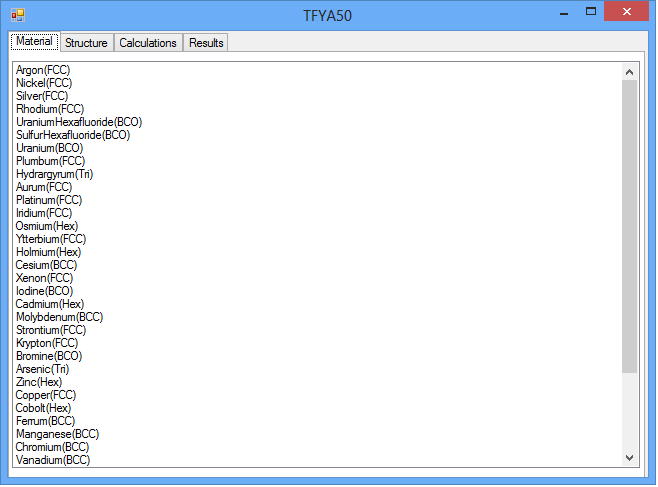
\includegraphics[width=0.7 \textwidth]{mat_tab.png}
	\caption{Interface for choosing matrial}
	\label{fig:mat_tab}
\end{figure}

Under the second tab is properties for setting up the dimensions and spacial properties of the simulation are found, see figure \ref{fig:struct_tab}. The default values, dependent on which element  that was chosen in step before, will be set here. The pre set values can be changed according to the users wishes.
\begin{figure}[h!]
	\centering
	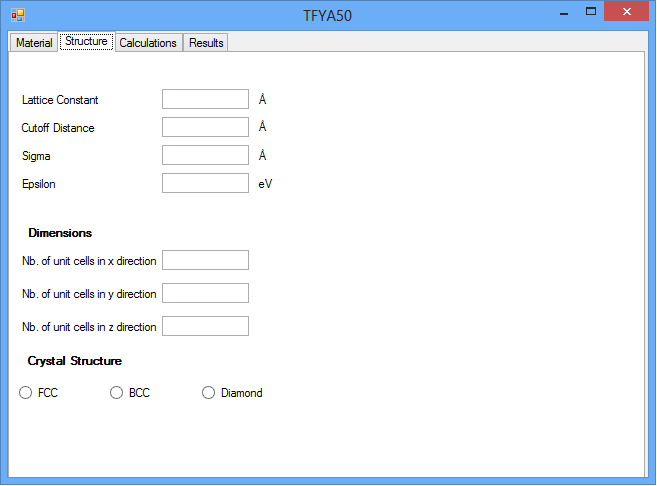
\includegraphics[width=0.7\textwidth]{struct_tab.png}
	\caption{Interface for setting material properties}
	\label{fig:struct_tab}
\end{figure}

The third tab consists of the simulation options. An overview is given in figure \ref{fig:calc_tab}. 
\begin{description}
	\item[Start calculations after \#timesteps] is the value at with point the average properties vil be started to accumulate
	\item[Run for \#timesteps] will be the amount of time steps for the simulation, tis multiplied with the timestep size will be the total runtime in femtoseconds for the simulation. 
	\item[Timestep size] will determine how long every time step should be in femtoseconds.
	\item[Include visualization] will when checked, produce a Matlab file  where the atomic movement can be seen
	\item[Save visualization every \#timestep] can be set so that not every point in the simulation is shed since that might take up to much storage space.
	\item[Save data every \#timestep] is used to decide at what interval property data should be saved.
	\item[Thermostat] will when checked activate the thermostat and an option to set the collision rate will also be given.
	\item[Collision rate] is set to a number between 0 and 1 and will be the chance of an atom colliding with the thermostat heat bath.
	\item[Temperature] is the starting temperature of the simulation. the atoms initial velocity will be scaled according to this. It will also be the temperature of the thermostat heat bath. The temperature is given in kelvin.
	\item[Use periodic boundary conditions] will when checked simulate the sample as continuous in the chosen directions. If boundary conditions are set an atom drifting away will jump over to the other side. By unchecking these conditions it is also possible to do surface simulations.
\end{description}
\begin{figure}[h!]
	\centering
	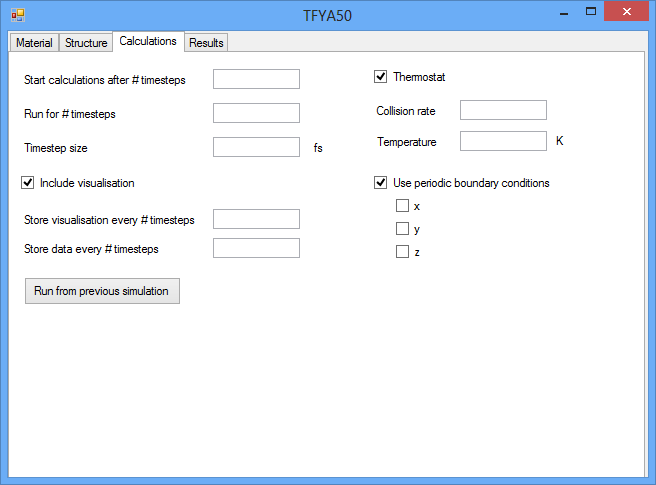
\includegraphics[width=0.7\textwidth]{calc_tab.png}
	\caption{Interface for setting calculation properties}
	\label{fig:calc_tab}
\end{figure}
	
The fourth and last tab is for starting the simulation and it will also provide the user with data on the simulation and present the average values for the listed properties when it's done as seen in figure \ref{fig:res_tab}.
\begin{figure}[h!]
	\centering
	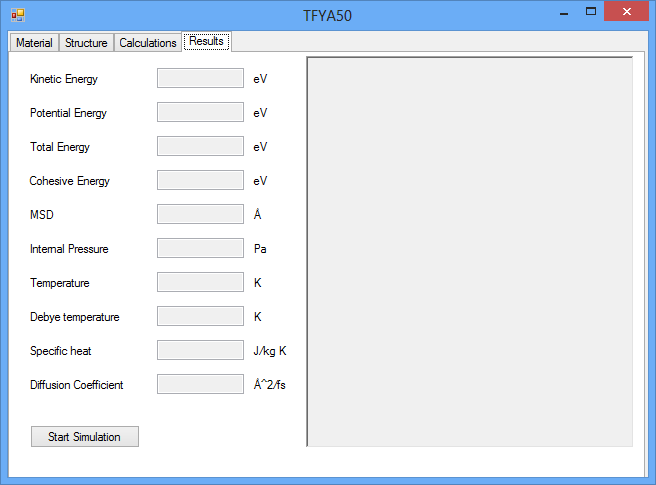
\includegraphics[width=0.7\textwidth]{res_tab.png}
	\caption{Interface for starting simulation and showing results}
	\label{fig:res_tab}
\end{figure}

When the simulation is running the program will be paused and when done a message will be send and the program will be unpaused. After running a simulation to end, a back2back file is produced to allow for multiple runs from the last state. In tab 3 simply choose run from previous simulation and choose the desired saved file.

Further more should a the user take notice and be cautious about that the program is producing new saving files with the same initial name every time it runs. This results in data being lost unless the user saves the back2back.txt, toto.txt, and titi.txt under different names or in a separate folder.

\subsection{Matlab}
Matlab is needed to produce the plots and to visualize the simulation. There are two Matlab files providing the programs that will take the data from toto.txt and titi.txt to calculate and plot the average values and the visualization respectively. To do so, launch Matlab and locate the folder with the Matlab files along with the txt files. In Matlab run the command ''plot\_data('toto.txt','\textbackslash{}t')'', where toto.txt is the name of the datafile and \textbackslash{}t is the delimiter. This allows the user to save files under different names and still being able to plot them. When running the command, nine plots will be produced. For the visualization part, simply run ''plot\_atoms()'' and the visualization will be loaded from the titi.txt file in the project folder.